\documentclass[border=10pt,tikz]{standalone}
\usepackage{tikz}
\usepackage{lmodern}
\usetikzlibrary{arrows.meta,positioning}

\begin{document}
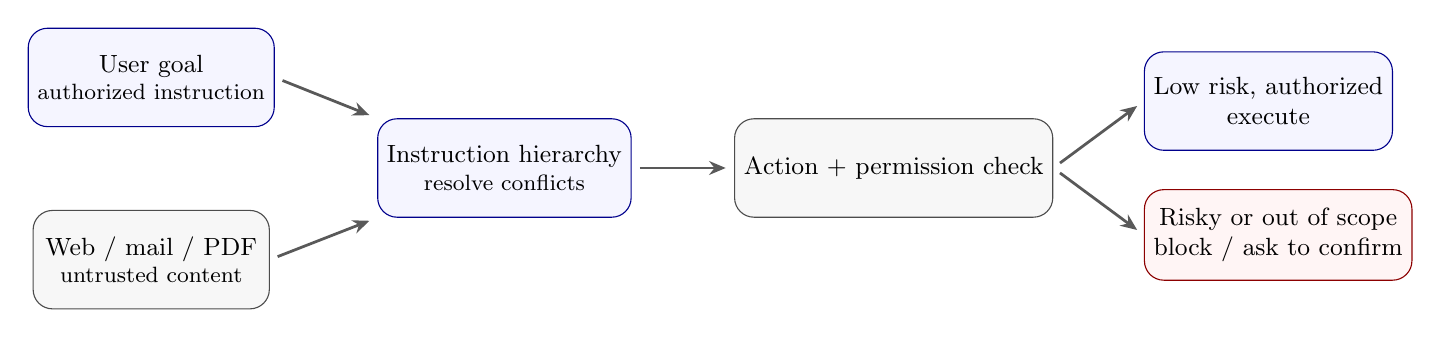
\begin{tikzpicture}[
  box/.style={draw=black!70,fill=black!3,rounded corners=7pt,minimum width=3.0cm,minimum height=1.25cm,align=center,font=\small},
  trusted/.style={draw=blue!55!black,fill=blue!4,rounded corners=7pt,minimum width=3.0cm,minimum height=1.25cm,align=center,font=\small},
  stop/.style={draw=red!55!black,fill=red!4,rounded corners=7pt,minimum width=3.0cm,minimum height=1.15cm,align=center,font=\small},
  arrow/.style={-{Stealth[length=6pt,width=5pt]},line width=1pt,black!65,shorten >=3pt,shorten <=3pt}
]
\node[trusted] (user) {User goal\\[-1pt]{\footnotesize authorized instruction}};
\node[box,below=1.05cm of user] (tool) {Web / mail / PDF\\[-1pt]{\footnotesize untrusted content}};
\node[trusted,right=1.3cm of user,yshift=-1.15cm] (policy) {Instruction hierarchy\\[-1pt]{\footnotesize resolve conflicts}};
\node[box,right=1.3cm of policy] (gate) {Action + permission check};
\node[trusted,right=1.15cm of gate,yshift=0.85cm] (run) {Low risk, authorized\\execute};
\node[stop,right=1.15cm of gate,yshift=-0.85cm] (confirm) {Risky or out of scope\\block / ask to confirm};
\draw[arrow] (user.east) -- (policy.north west);
\draw[arrow] (tool.east) -- (policy.south west);
\draw[arrow] (policy) -- (gate);
\draw[arrow] (gate.east) -- (run.west);
\draw[arrow] (gate.east) -- (confirm.west);
\end{tikzpicture}
\end{document}
